\chapter{Cálculos}
\markboth{Módulo 2}{}

\section*{Habilidades do SAEB}

\begin{itemize}
\item Calcular o resultado de adições ou subtrações, envolvendo números
naturais de até 6 ordens.

\item Calcular o resultado de multiplicações ou divisões, envolvendo números
naturais de até 6 ordens.

\item Associar o quociente de uma divisão com resto zero de um número
natural de até 6 ordens por 2, 3, 4, 5 e 10 às ideias de metade, terça,
quarta, quinta e décima parte.

\item Resolver problemas de adição ou de subtração, envolvendo números
naturais de até 6 ordens, com os significados de juntar, acrescentar,
separar, retirar, comparar ou completar.

\item Resolver problemas de multiplicação ou de divisão, envolvendo números
naturais de até 6 ordens, com os significados de formação de grupos
iguais (incluindo repartição equitativa e medida), proporcionalidade ou
disposição retangular.
\end{itemize}

\subsection{Habilidades da BNCC}

\begin{itemize}
\item EF03MA06, EF03MA07, EF03MA08.
\end{itemize}

%\conteudo{ Assim como todos os conteúdos que envolvem as quatro operações básicas, este módulo é essencial e seu estudo deve ser feito com tempo para bastante treino. Relembre com os alunos cada detalhe e os algoritmos de adição, subtração, multiplicação e divisão, dando  ênfase à divisão, que geralmente é o maior desafio enfrentado pelos alunos. }
\pagebreak

\conteudo{
\begin{itemize}
\item [ ] \textsc{Adição}
\end{itemize}
\begin{center}
\noindent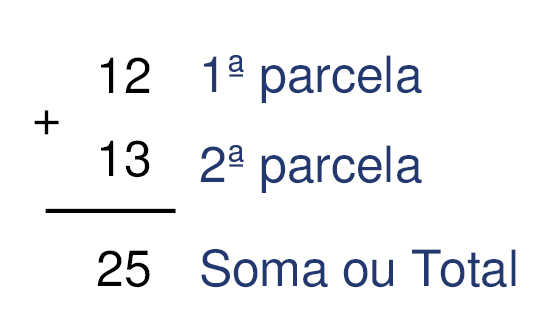
\includegraphics[width=.3\textwidth]{./media/image10.png}
\end{center}

\begin{itemize}
\item [ ] \textsc{Subtração}
\end{itemize}
\begin{center}
\noindent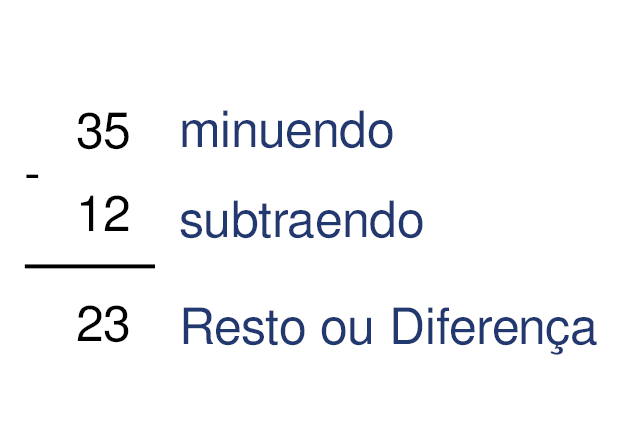
\includegraphics[width=.3\textwidth]{./media/image11.png}
\end{center}

\begin{itemize}
\item [ ] \textsc{Multiplicação}
\end{itemize}
\begin{center}
\noindent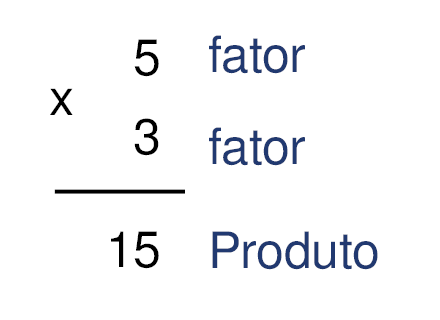
\includegraphics[width=.3\textwidth]{./media/image12.png}
\end{center}

\begin{itemize}
\item [ ] \textsc{Divisão}
\end{itemize}
\begin{center}
\noindent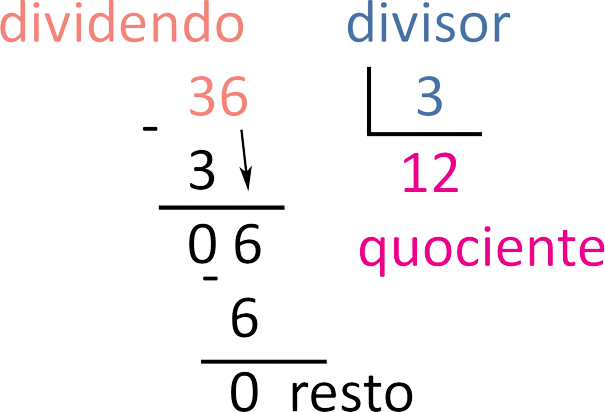
\includegraphics[width=.3\textwidth]{./media/image13.png}
\end{center}
}

\pagebreak 

\section*{Atividades}

\num{1} Adicione ou subtraia para obter o número desejado.

\begin{escolha}

\item
  Transforme 262 em 362.\\
\reduline{Adicionar 100.\hfill}
\linhas{2}

\item
  Transforme 1.100 em 1.000.\\
\reduline{Subtrair 100.\hfill}
\linhas{2}

\item
  Transforme 238 em 239.\\
\reduline{Adicionar 1.\hfill}
\linhas{2}
\end{escolha}

\num{2} Utilize os sinais menor que (\textbf{\textless{}}), maior que (\textbf{\textgreater{}}) ou igual a
(\textbf{=}) em cada situação para comparar as quantidades representadas.\bigskip

\begin{minipage}{.5\textwidth}
\begin{escolha}
\item
  7 \reduline{Menor que, \textless{}} 14
\item
  21 \reduline{Maior que, \textgreater{}} 5
\item
  1 + 3 \reduline{Igual a, =} 2 + 2
  \end{escolha}
  \end{minipage}
\begin{minipage}{.5\textwidth}
  \begin{escolha}[start=4]
\item
  5 + 2 \reduline{Maior que, \textgreater{}} 7 -- 1
\item
  20 -- 1 \reduline{Igual a, =} 19
\item
  Treze \reduline{Menor que, \textless{}} quinze
\end{escolha}
\end{minipage}

\pagebreak

\num{3} Ligue a operação na coluna 1 ao seu resultado na coluna 2.

\begin{multicols}{2}
84 + 12

60 -- 23

67 -- 58

50 -- 2 x (5 + 15) + 2

2 + 8 -- 2 x (1 + 2)

37

9

96

4

12
\end{multicols}
%\coment{Explore ao máximo com os alunos o conceito de quais operações devem ser realizadas primeiro e, assim, ajude na fixação desse conceito.
\coment{Respostas: 84 + 12 = 96; 60 - 23 = 37; 67 - 58 = 9; 50 - 2 x (5 + 15) + 2 = 50 - 40 + 2 = 12; 2 + 8 - 2 x (1 + 2) = 2 + 8 - 6 = 4}

\num{4} Observe atentamente a figura dada e, em seguida, responda ao que se pede em cada item.


\begin{figure}[htpb!]
\centering
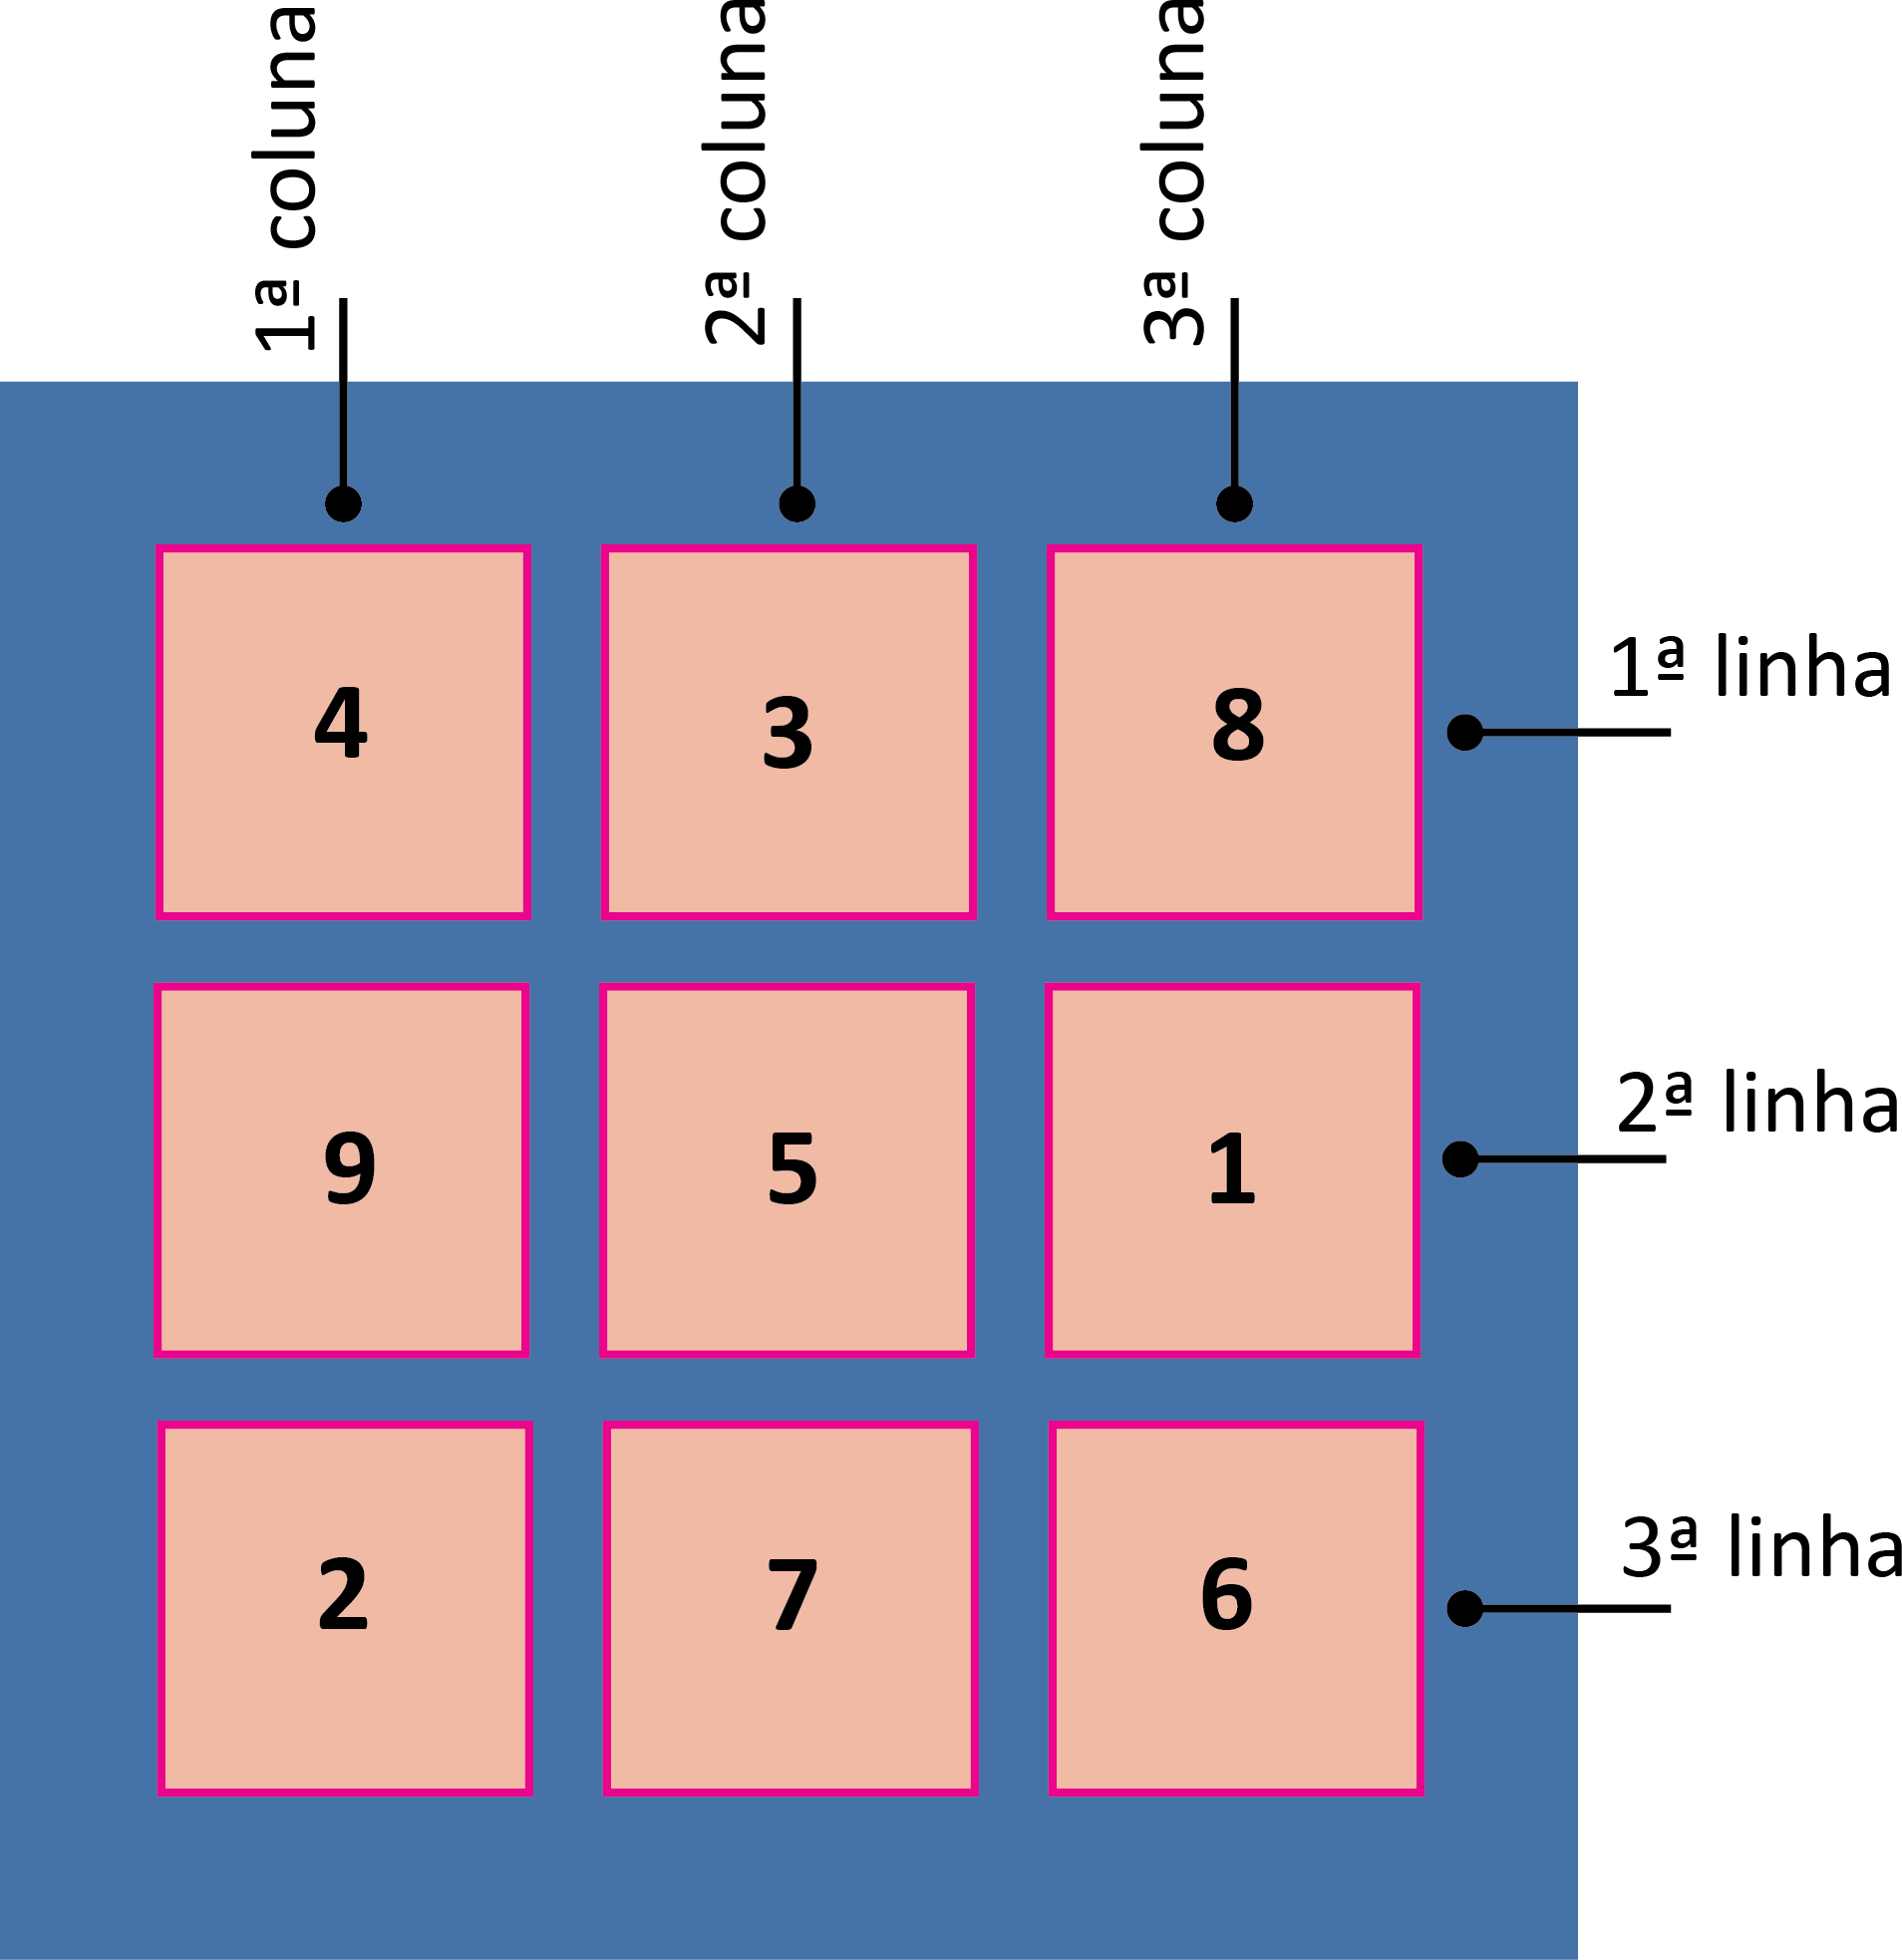
\includegraphics[width=.5\textwidth]{./media/image14.png}
\end{figure}

\begin{escolha}
\item Calcule a soma de todos os números que estão na 1ª coluna.
\reduline{4 + 9 + 2 = 15.\hfill}
\linhas{1}

\pagebreak
\item Calcule a soma de todos os números que estão na 2ª coluna.
\reduline{3 + 5 + 7 = 15.\hfill}
\linhas{1}

\item Calcule a soma de todos os números que estão na 3ª coluna.
\reduline{8 + 1 + 6 = 15.\hfill}
\linhas{1}

\item O que você percebe ao comparar os resultados das somas dos números de cada coluna?
\reduline{O resultado de todas as somas apresentam resultado igual a 15.\hfill}
\linhas{1}

\item Calcule a soma dos números que estão na 1ª linha.
\reduline{4 + 3 + 8 = 15.\hfill}
\linhas{1}

\item Calcule a soma dos números que estão na 2ª linha.
\reduline{9 + 5 + 1 = 15.\hfill}
\linhas{1}

\item Calcule a soma dos números que estão na 3ª linha.
\reduline{2 + 7 + 6 = 15.\hfill}
\linhas{1}

\item O que você percebe quando compara os resultados da soma dos números de cada linha?
\reduline{O resultado de todas as somas apresentam resultado igual a 15.\hfill}
\linhas{1}
\end{escolha}

\num{5} Vicente vendeu 6 sorvetes de chocolate, 8 de morango, 3
de groselha e 5 de creme. Quantas unidades de sorvete Vicente vendeu?
\begin{figure}[htpb!]
\centering
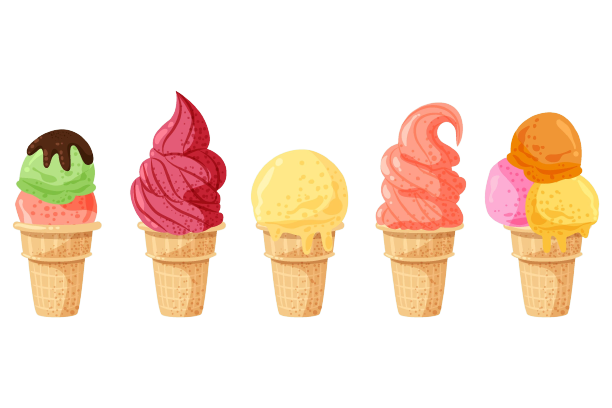
\includegraphics[width=.5\textwidth]{./media/image14a.png}
\end{figure}

\reduline{Vicente vendeu 6 + 8 + 3 + 5 = 22. \hfill}
\linhas{1}

\num{6} A receita de um bolo pede para colocar 260 g de
farinha de trigo e misturar com ovos, açúcar e leite. 
Em seguida, solicita o acréscimo de mais 135 g de farinha de trigo. 
Calcule a quantidade total de farinha utilizada nesta receita?

\begin{figure}[htpb!]
\centering
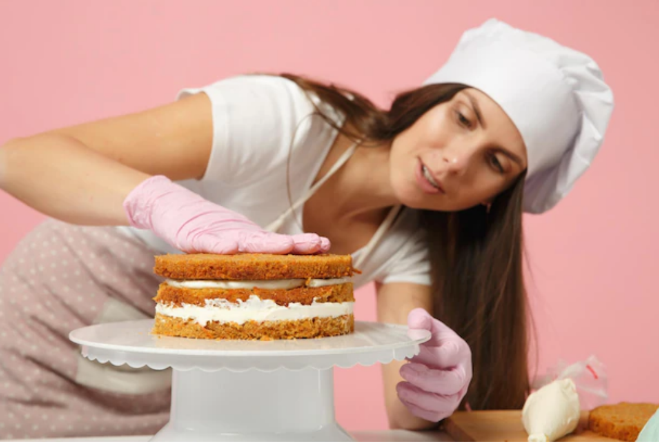
\includegraphics[width=.5\textwidth]{./media/image15.png}
\end{figure}
\reduline{260 + 135 = 395 g.\hfill}
\linhas{3}

\num{7} Raquel adora confeitaria. Por isso, 
decidiu começar uma pequena empresa de doces para festas. 
Para o próximo final de semana, ela recebeu a seguinte 
encomenda por mensagem de texto em seu celular:

\begin{myquote}
\centering
\textbf{Encomenda para a festa da Maria}

\begin{itemize}
\centering
\item [ ] 275 brigadeiros

\item [ ] 165 beijinhos

\item [ ] 245 cajuzinhos
\end{itemize}
\end{myquote}

Calcule o total de unidades de doces que Raquel terá que fazer para entregar essa encomenda.
\reduline{275 + 165 + 245 = 685.\hfill}
\linhas{3}

\num{8} Complete o quadro, transformando as adições em multiplicações. Em seguida, encontre o resultado.

\begin{longtable}[]{@{}lll@{}}
\toprule
\hline
\vspace{1ex}
\textbf{Adição de parcelas iguais} & \textbf{Multiplicação} & \textbf{Resultado}\tabularnewline
\midrule
\endhead
\hline
\vspace{1ex}
8 + 8 + 8 & 3 x 8 & 24\tabularnewline
\hline
\vspace{1ex}
10 + 10 + 10 + 10 + 10 & \rosa{5 x 10} & \rosa{50}\tabularnewline
\hline
\vspace{1ex}
6 + 6 + 6 + 6 & \rosa{6 x 4} & \rosa{24}\tabularnewline
\hline
\vspace{1ex}
5 + 5 + 5 + 5 + 5 + 5 + 5 & \rosa{5 x 7} & \rosa{35}\tabularnewline
\hline
\vspace{1ex}
12 + 12 + 12 + 12 + 12 & \rosa{12 x 5} & \rosa{60}\tabularnewline
\bottomrule
\end{longtable}

\pagebreak
\num{9} João possui uma distribuidora de ovos. Hoje, ele recebeu 15 caixas  
que contém individualmente 252 ovos. Para vendê-los, João utilizou embalagens de
12 unidades. Quantas embalagens são necessárias para que João venda 
todos os ovos que recebeu?

\begin{figure}[htpb!]
\centering
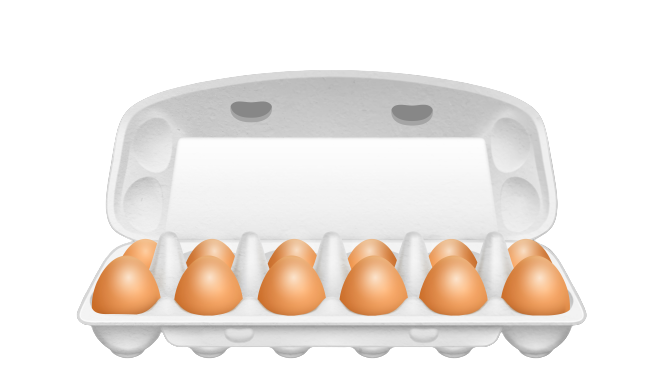
\includegraphics[width=.5\textwidth]{./media/image16a.png}
\end{figure}
\reduline{(15 x 252) : 12 = 315.\hfill}
%\reduline{É sempre recomendado escrever a expressão formada pela interpretação do enunciado, pois assim os alunos vão aprendendo a transformar textos em linguagem matemática.\hfill}

\num{10} A mãe de Beatriz comprou uma caixa de bombons para presentear os quatro filhos. 
Na caixa, os bombons estavam distribuídos em 8 fileiras de 9 unidades. 

\begin{figure}[htpb!]
\centering
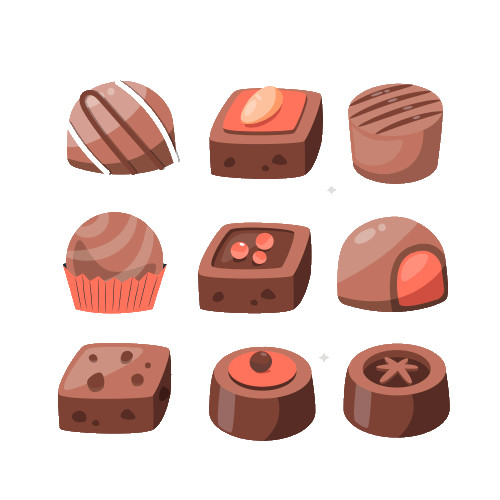
\includegraphics[width=.4\textwidth]{./media/image16b.jpeg}
\end{figure}

Calcule a quantidade de bombons que cada filho deve receber, caso todos ganhem a mesma quantidade.
\reduline{Beatriz receberá 18 bombons, assim como seus irmãos: (8 x 9) : 4 = 18.\hfill}
\linhas{1}


\num{11} Brenda se deparou com uma divisão em sua prova de matemática. 
Nela, o número 5.192 era o dividendo, e o número 22 era o divisor. 
Calcule o quociente, sabendo que Brenda acertou o cálculo.

\begin{figure}[htpb!]
\centering
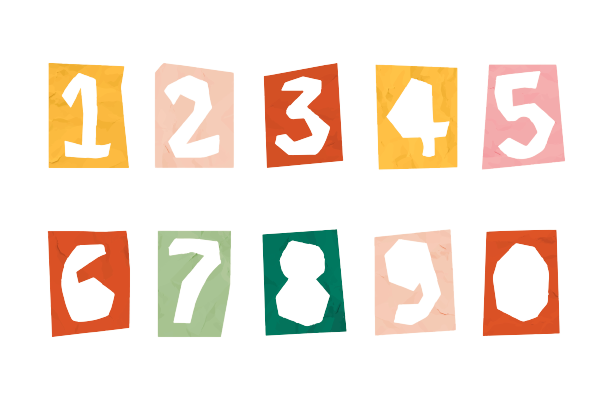
\includegraphics[width=.7\textwidth]{./media/image16c.png}
\end{figure}
%\coment{Explore também divisões com dividendos maiores.}
\reduline{5.192 : 22 = 236.\hfill}
\linhas{2}

\num{12} Complete cada frase com a palavra ``dobro'' ou com a palavra ``triplo''.

\begin{escolha}
\item
  O \reduline{dobro\hfill} de 10 é 20.
\item
  O \reduline{triplo\hfill} de 6 é 18.
\item
  O \reduline{dobro\hfill} de 7 é 14.
\item
  O \reduline{triplo\hfill} de 8 é 24.
\end{escolha}

\pagebreak
\num{13} No quadro branco da professora Adriana, foram escritos os números a seguir:

%Construir uma figura conforme a abaixo. Os números importam e devem ser os mesmos.

\vspace{2em}
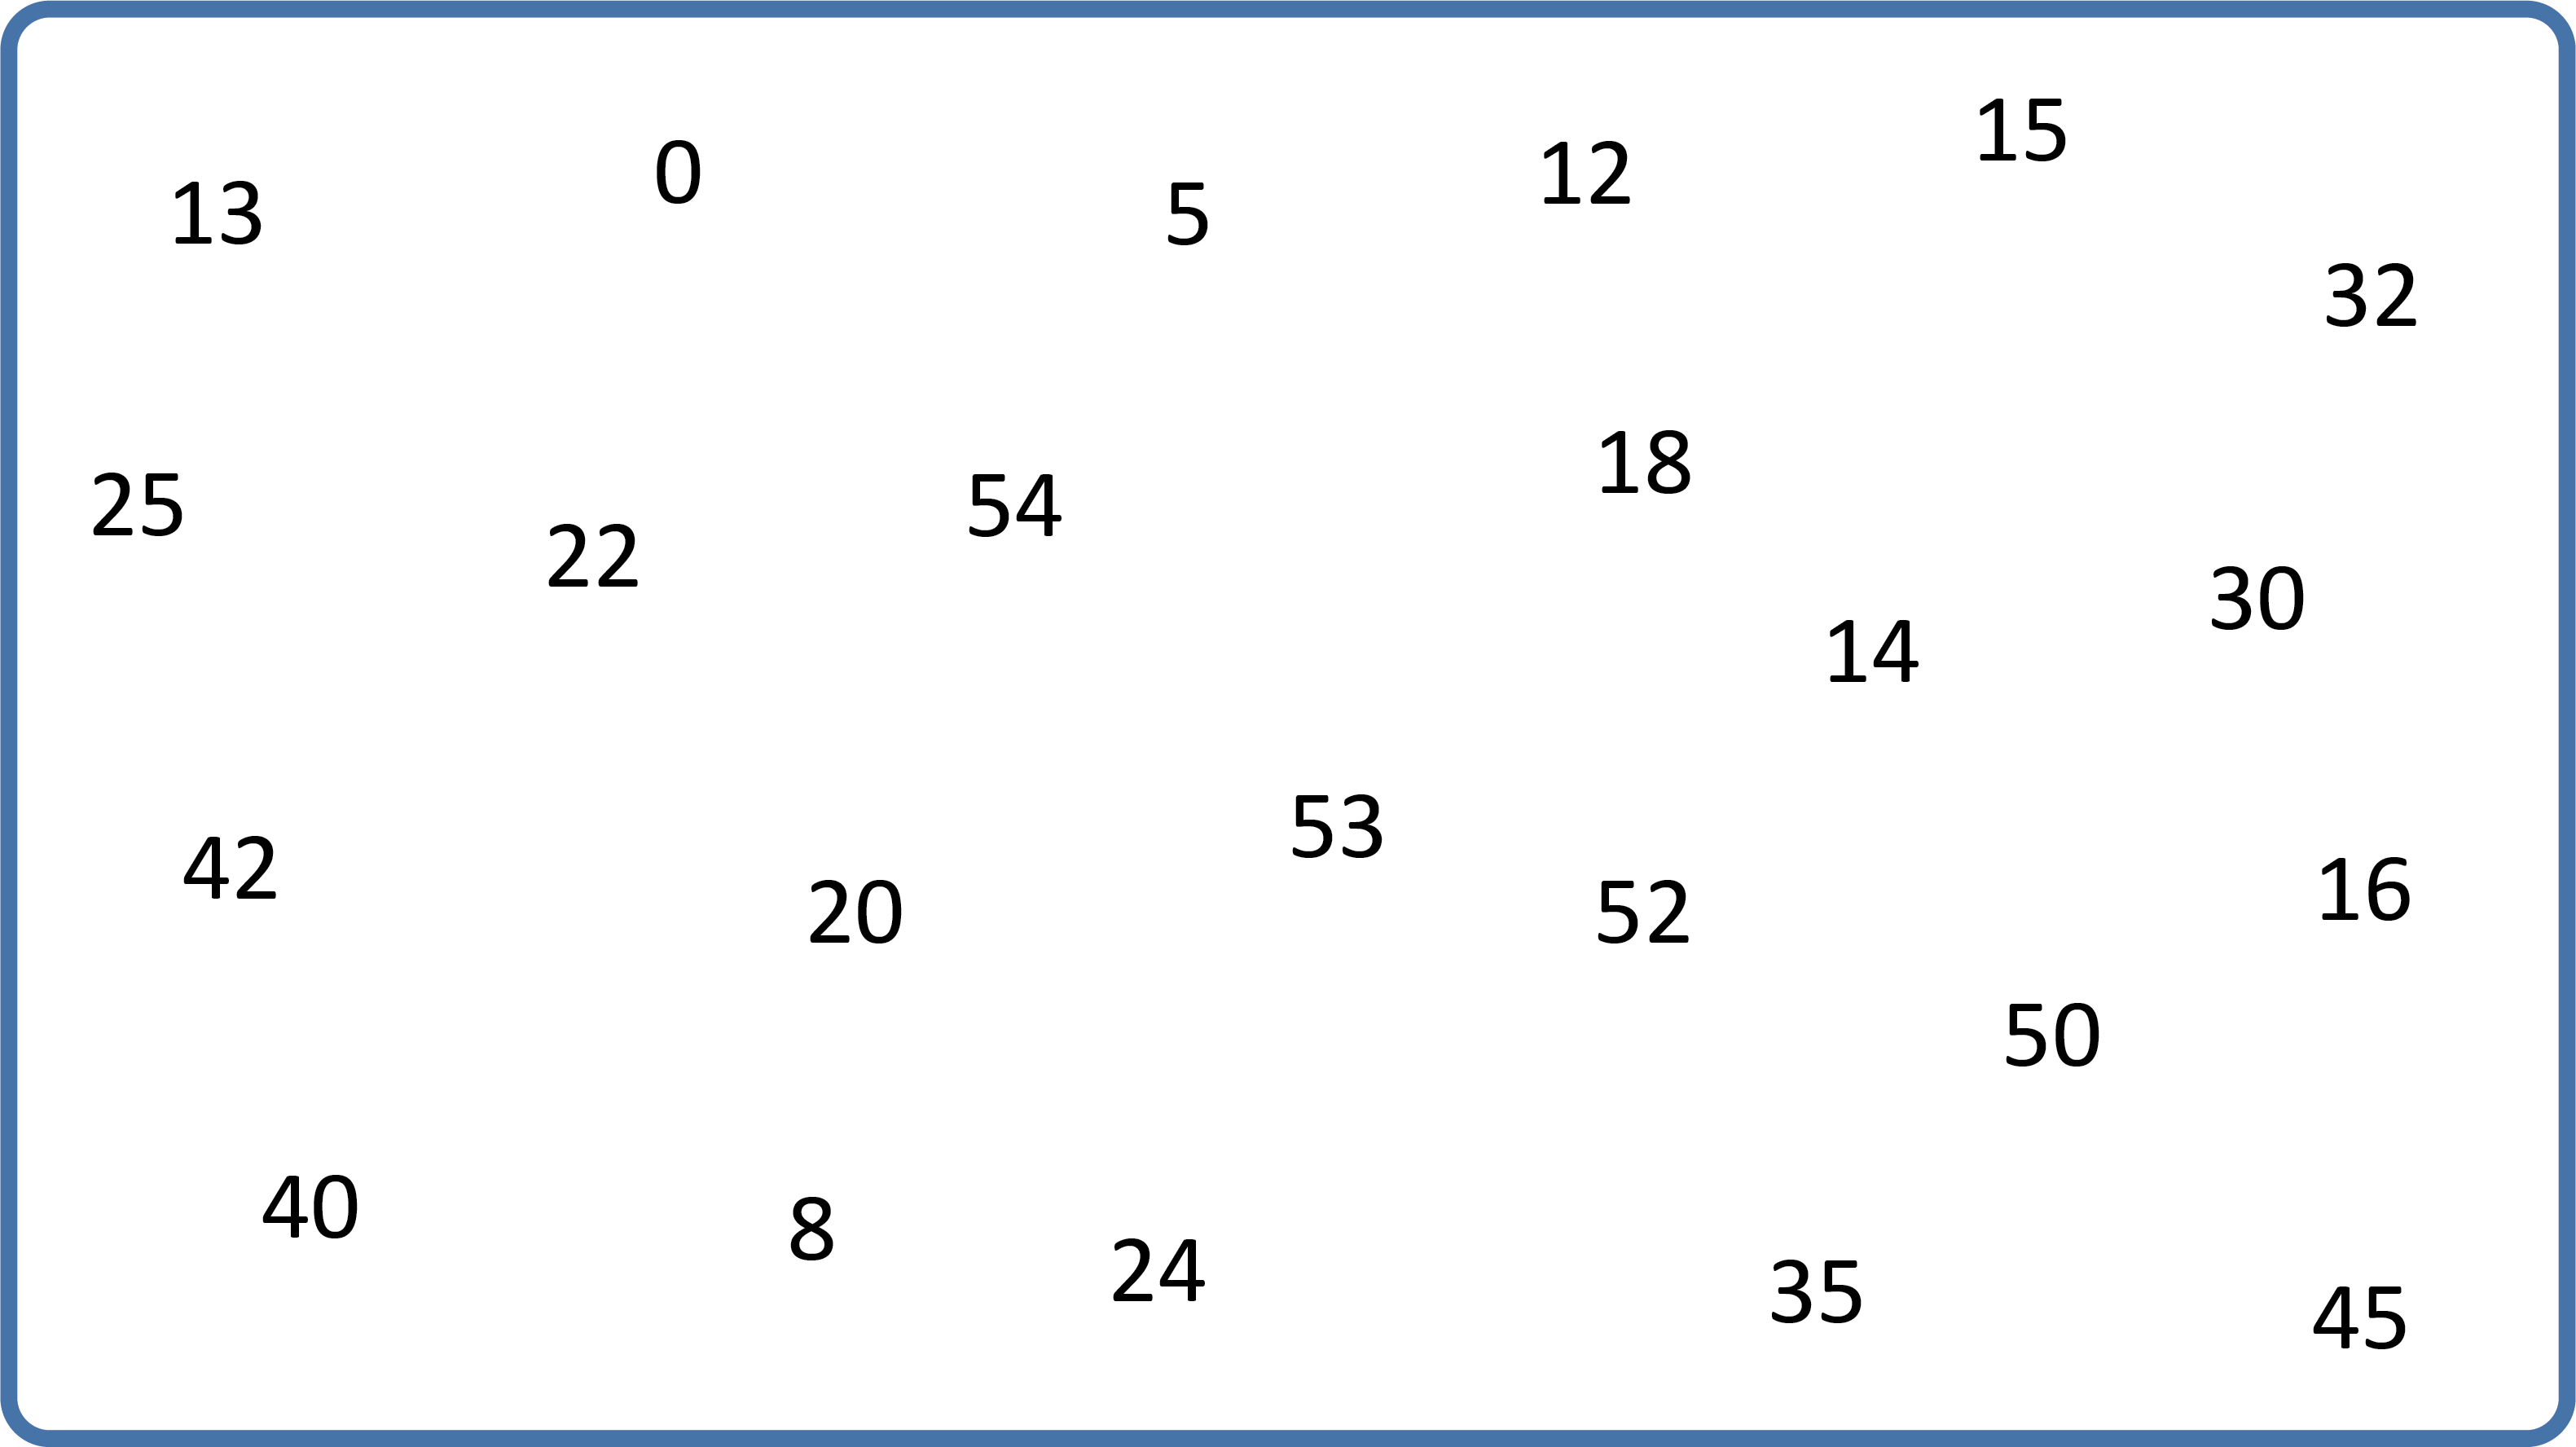
\includegraphics[width=\textwidth]{./media/image25.png}
\vspace{2em}

Circule aqueles que fazem parte da tabuada do 3.
\reduline{12; 15; 54; 42; 24; 45.\hfill}
\linhas{6}


\begin{comment}
\num{12} Observe a conversa entre Rebeca, Raquel e Renata no sítio do avô de Rebeca.

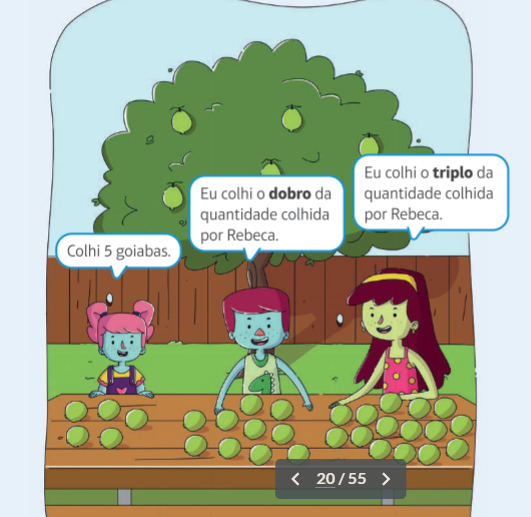
\includegraphics[width=4.42538in,height=4.30871in]{./media/image24.png}

%Fazer uma ilustração nos moldes dessa, colocando o nome de cada menina na lateral da mesa a frente delas. Na fala de Renata trocar Rebeca por Raquel. Trocar goiabas por maçãs no texto e nas frutas em cima da mesa. Trocar a palavra dobro na historinha por triplo e aumentar o número de frutas da mesa para 15 na frente dessa menina. Trocar a quantidade frutas na frente da terceira menina para 45.

\begin{escolha}
\item Qual a quantidade de maçãs que Rebeca colheu?
\reduline{5\hfill}
\linhas{2}

\item Calcule a quantidade de maçãs que Raquel colheu?
\reduline{3 x 5 = 15\hfill}
\linhas{2}

\item Qual a quantidade de maçãs que Renata colheu?
\reduline{3 x 15 = 45\hfill}
\linhas{2}
\end{escolha}
\end{comment}

\pagebreak

\section*{Treino}

\num{1} Uma costureira recebeu uma encomenda para colocar 6 botões em
cada uma das 9 camisas que José utiliza para trabalhar. Quantos botões
ela precisará no total para concluir a tarefa?

\begin{figure}[htpb!]
\centering
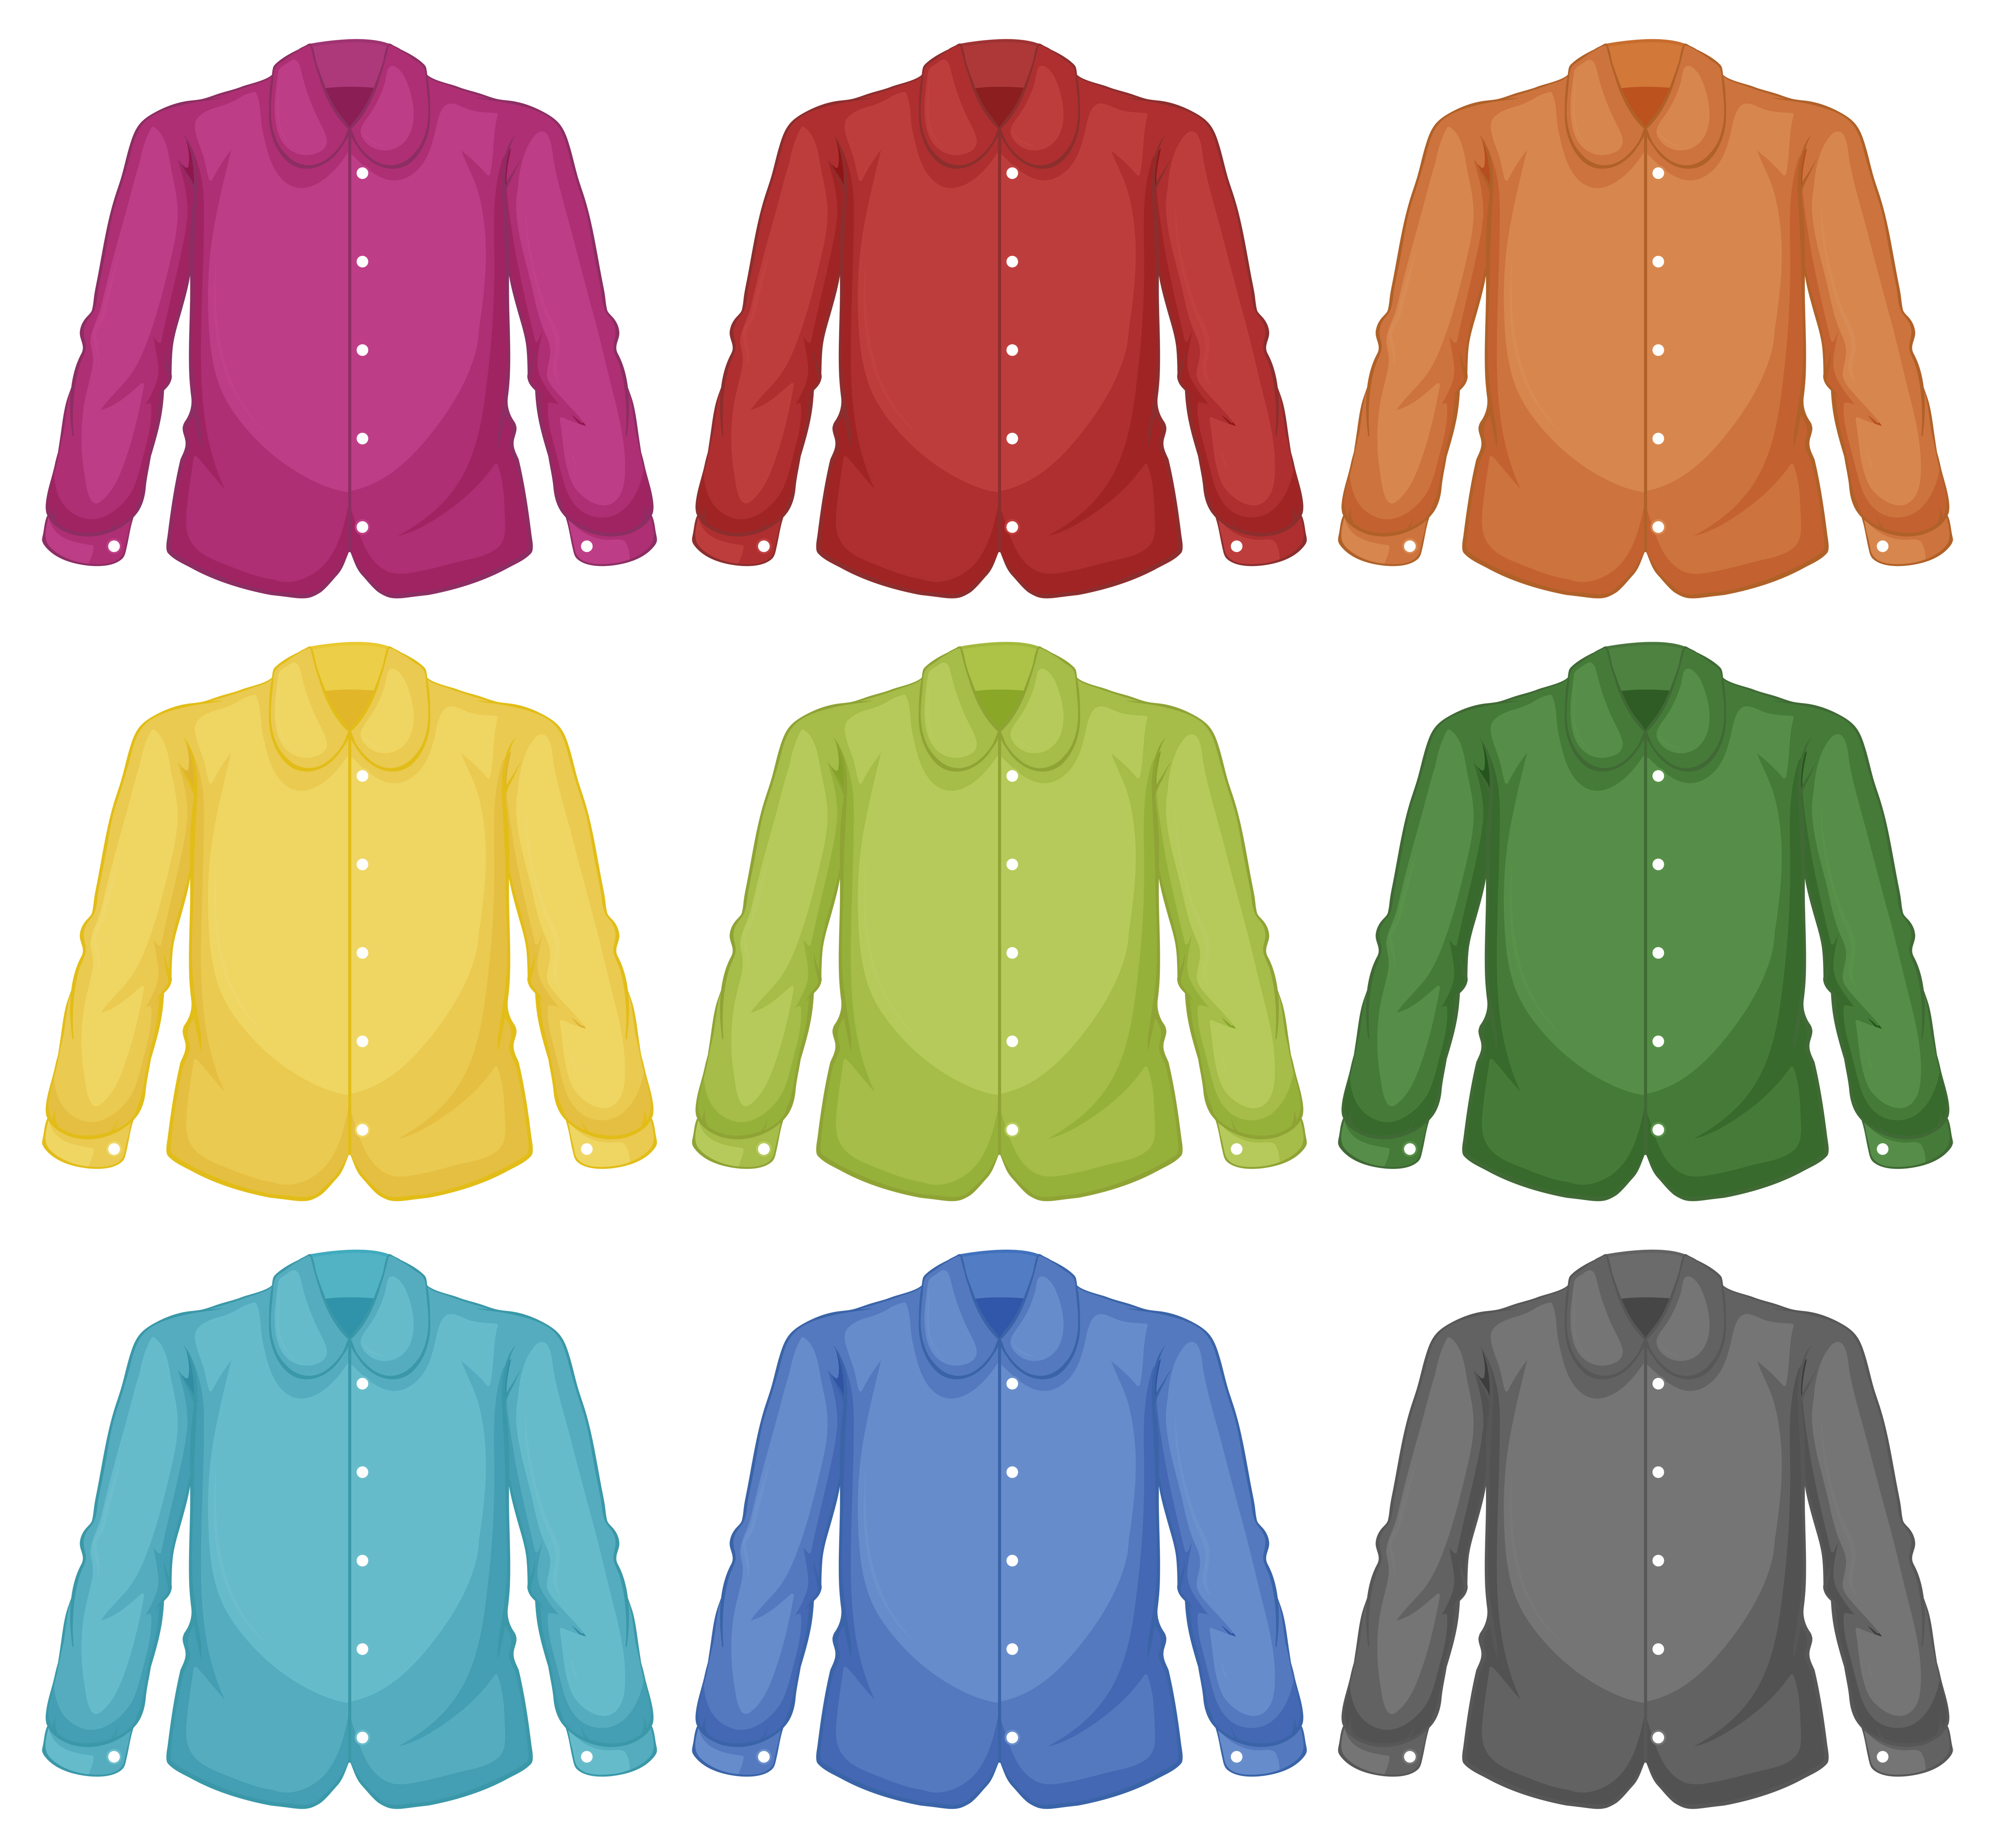
\includegraphics[width=.8\textwidth]{./media/image16d.jpeg}
\end{figure}

\begin{escolha}
    \item 6.
    \item 9.
    \item 15.
    \item 54.
\end{escolha}

\pagebreak

\num{2} Para uma festa familiar, a mãe de Josué comprou 12 fardos de
suco como os representados pela imagem a seguir. Quantas garrafas de suco foram compradas para a festa? 
%Incluir imagem disponível em https://br.freepik.com/vetores-gratis/latas-em-embalagens-plasticas_11684670.htm#query=six%20pack%20soda&position=0&from_view=search&track=robertav1_2_sidr

\begin{minipage}{.5\textwidth}
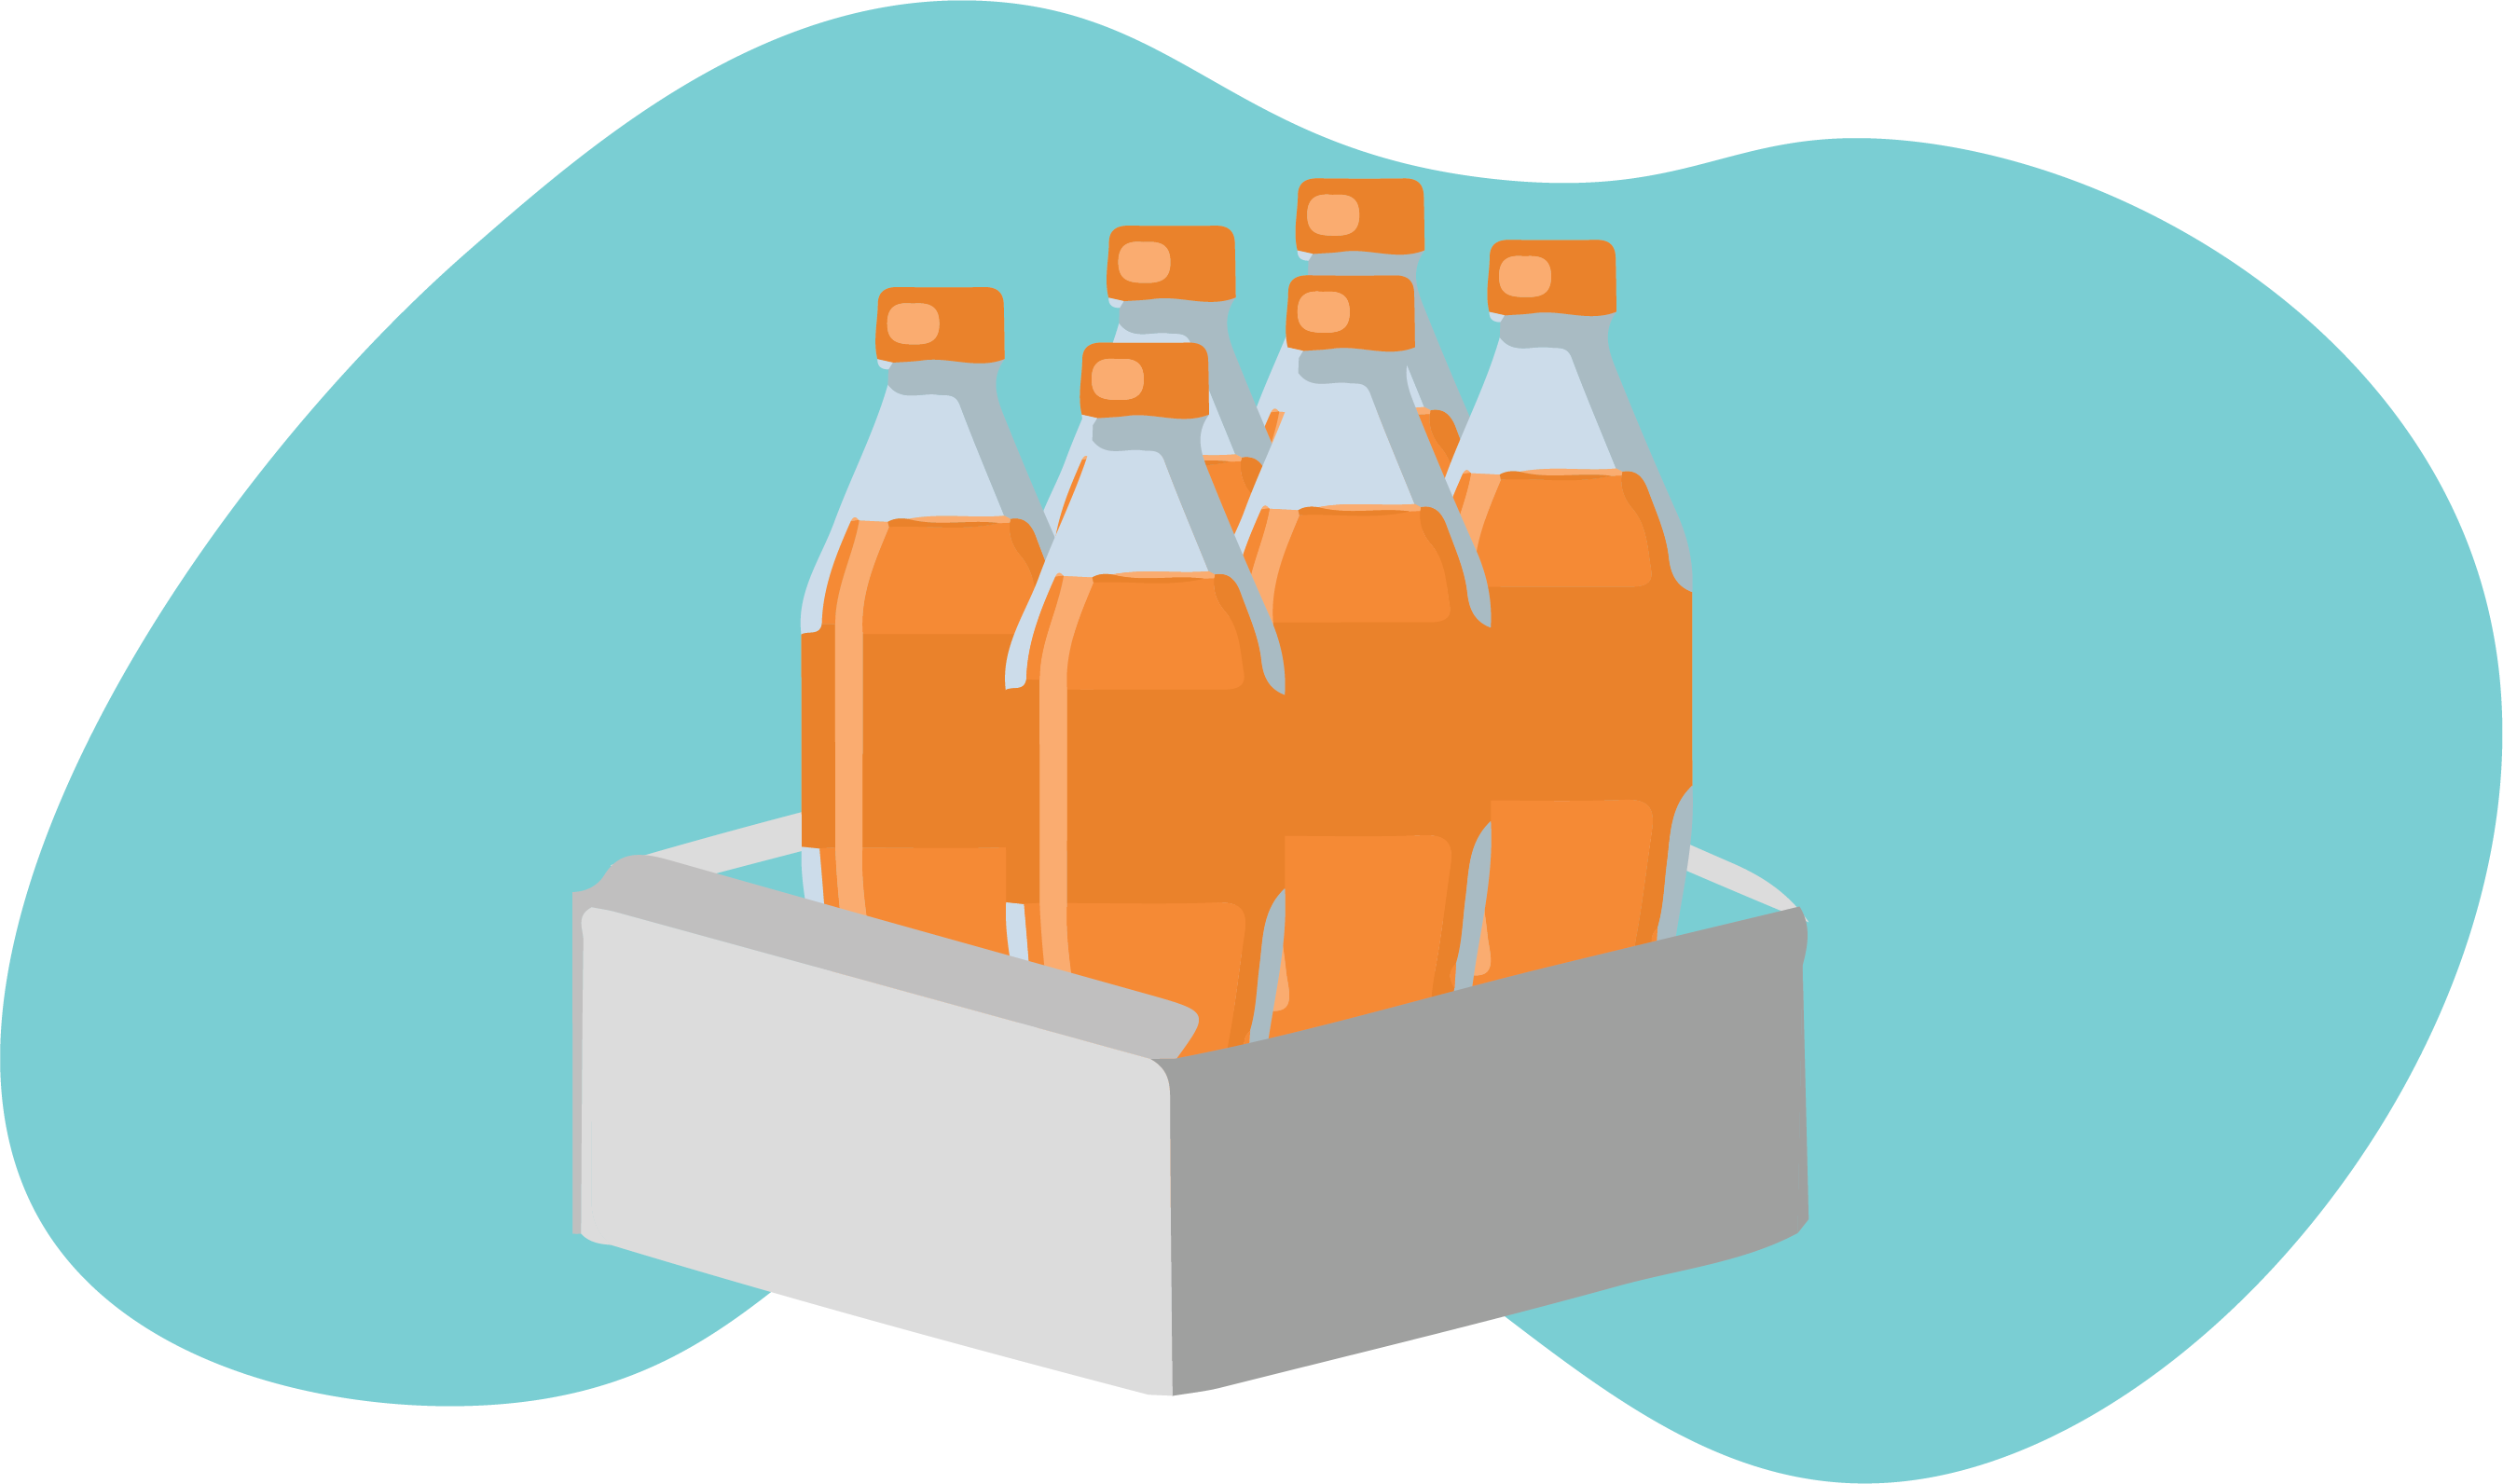
\includegraphics[width=\textwidth]{./media/image26.png}
\end{minipage}
\begin{minipage}{.5\textwidth}
\begin{escolha}
\item
  6 garrafas de suco.
\item
  12 garrafas de suco.
\item
  72 garrafas de suco.
\item
  144 garrafas de suco.
\end{escolha}
\end{minipage}

\num{3} Um campeonato interno de basquete será promovido na escola em que Carlos
estuda. Pelas regras, cada time deverá ter 5 jogadores titulares e mais 3 reservas. Considerando que serão formados 6 times, qual é a quantidade de alunos que poderão participar do campeonato?

\begin{figure}[htpb!]
\centering
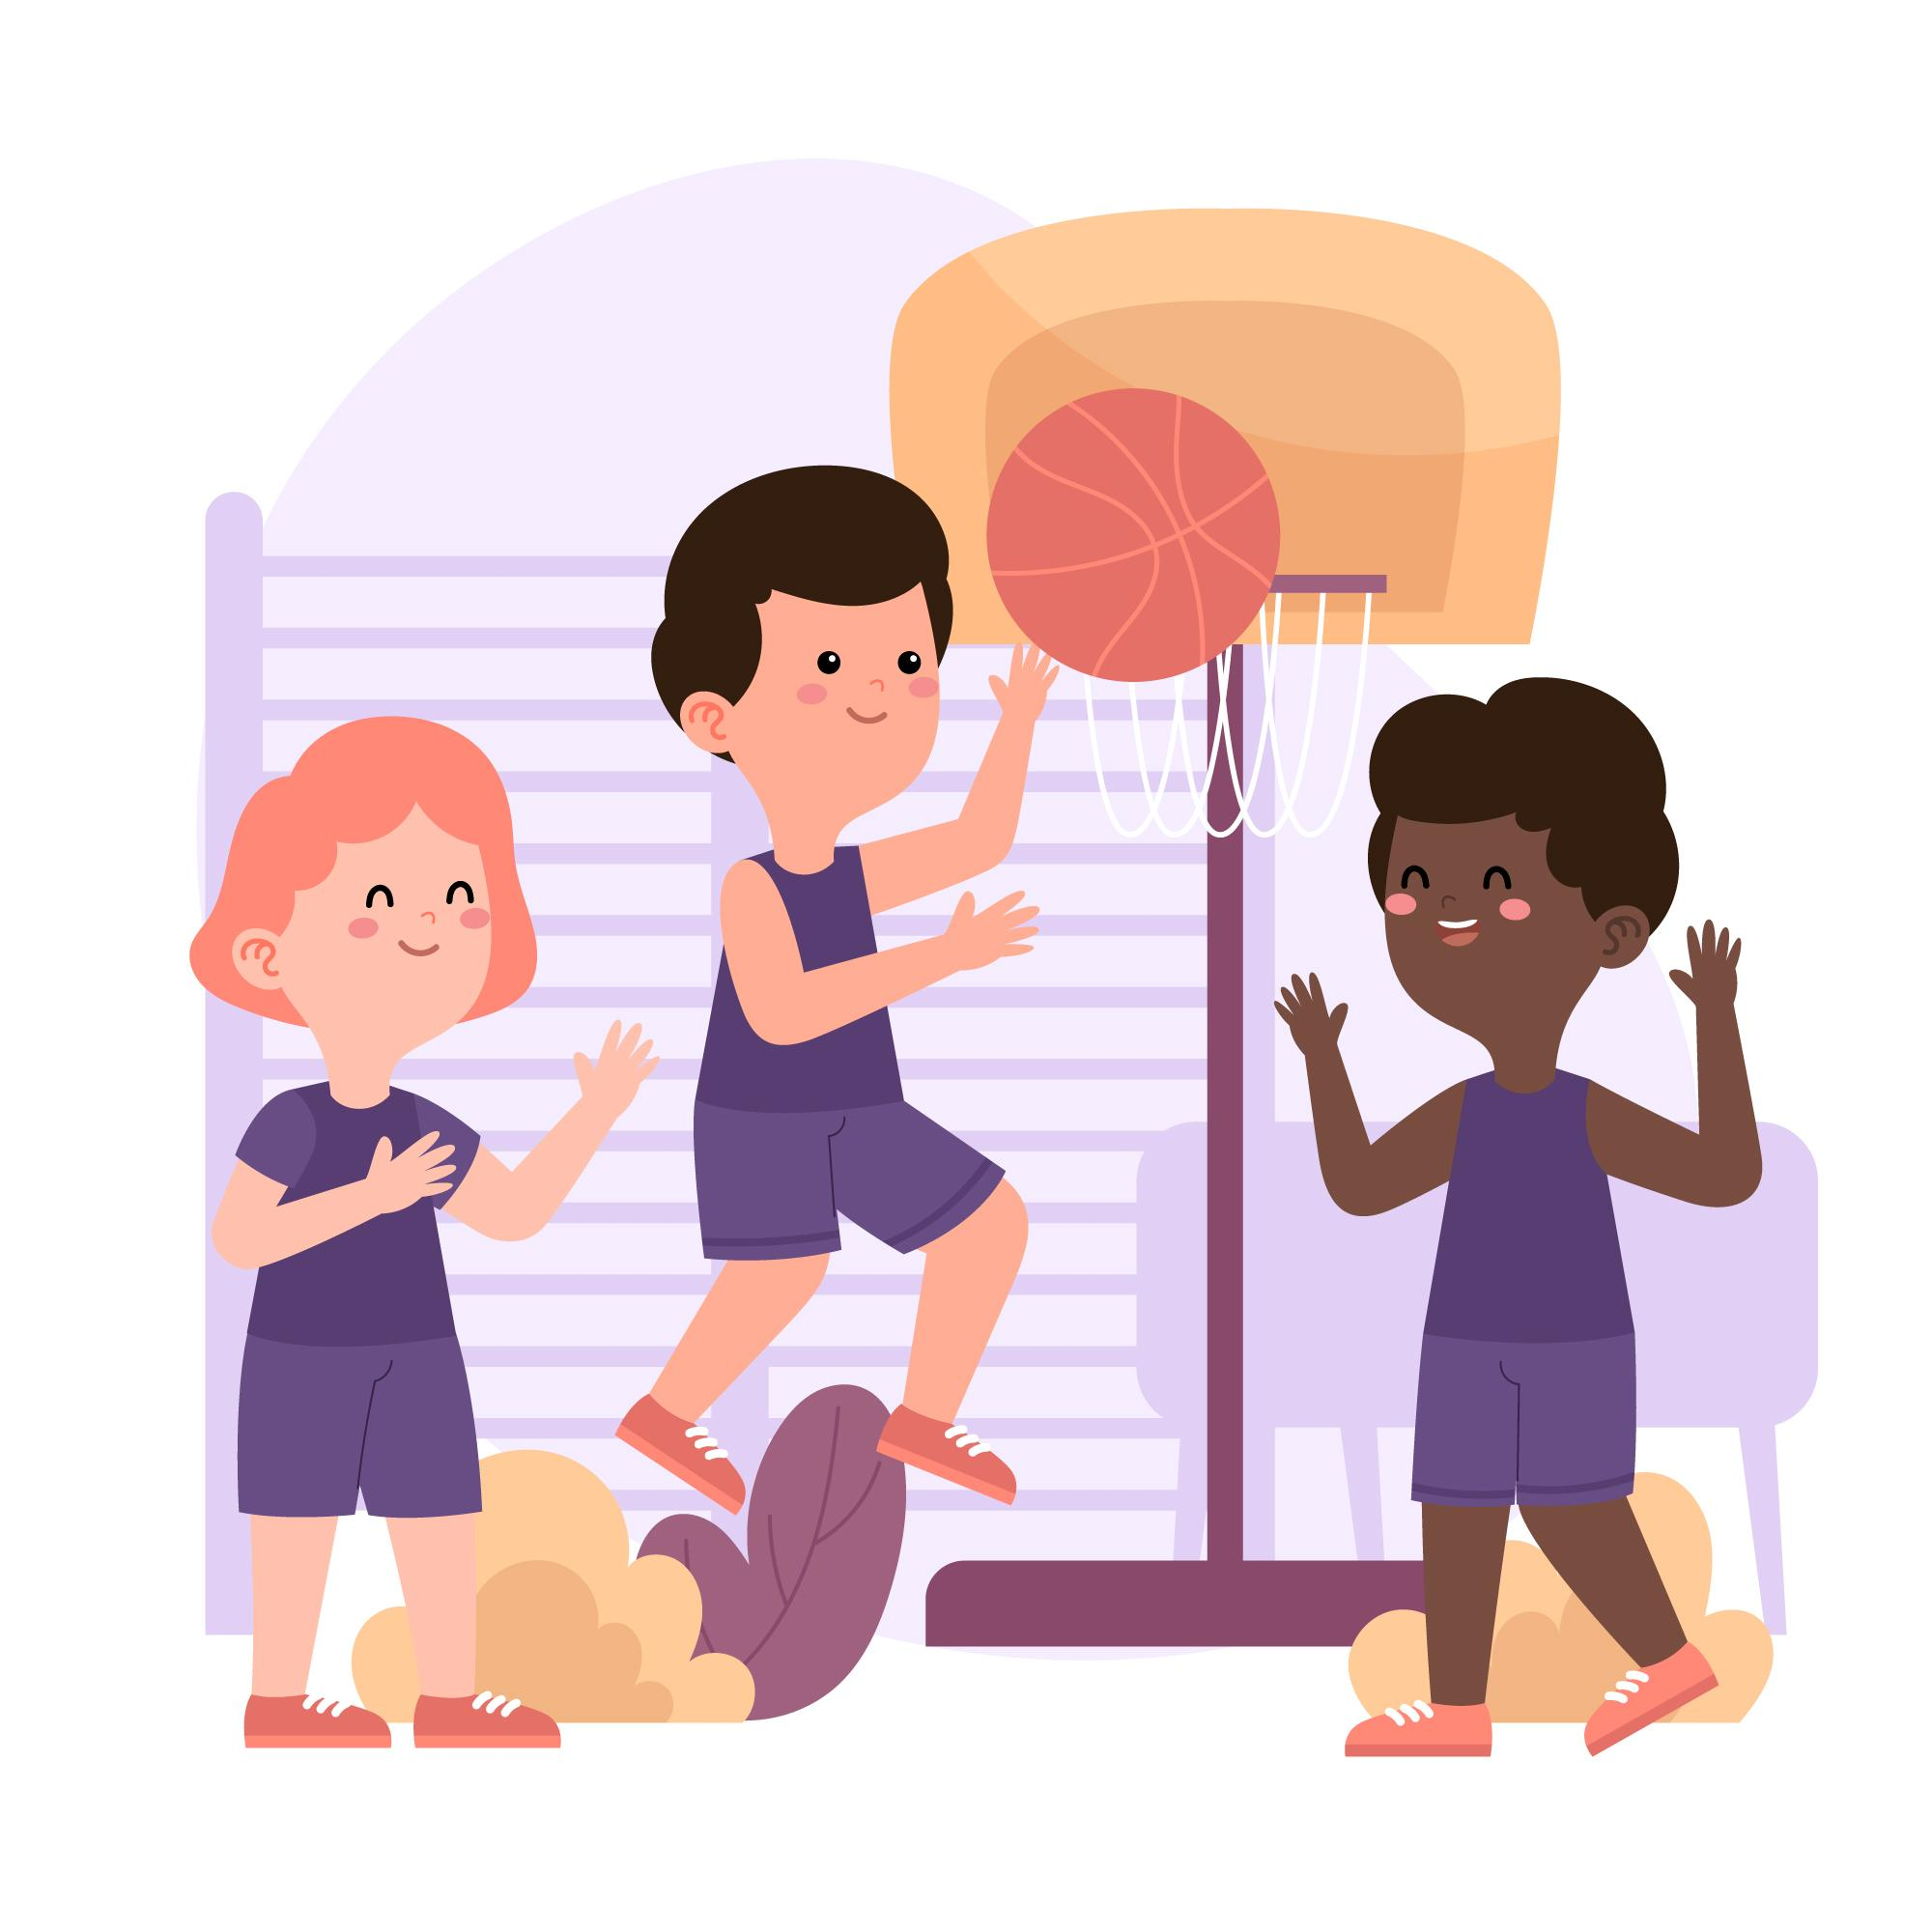
\includegraphics[width=.6\textwidth]{./media/image16e.jpeg}
\end{figure}

\begin{multicols}{2}
\begin{escolha}
\item
  18.
\item
  30.
\item
  36.
\item
  48.
\end{escolha}
\end{multicols}
